
%\tikzstyle{cor} = []
\tikzstyle{fonte} = [font=\footnotesize]

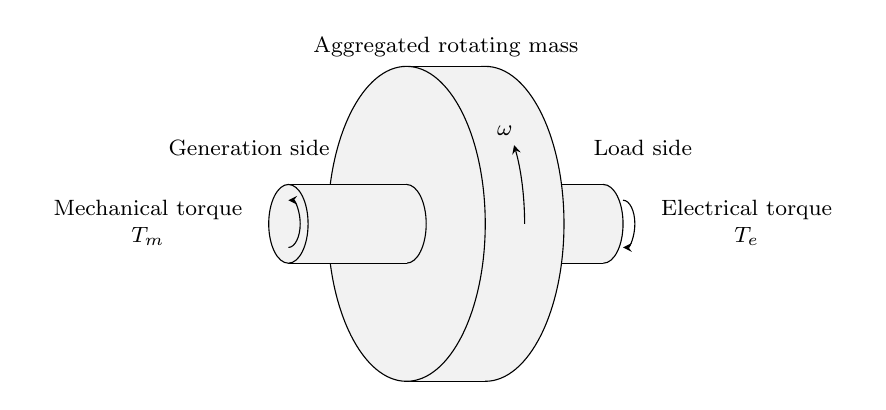
\begin{tikzpicture}[>=stealth]
 
    % shaft load end
    \draw [fill=black!5] (2,0) circle [x radius=0.25cm, y radius=0.5cm];
    \fill [black!5] (0,-0.5) rectangle (2,0.5);
    \draw [] (2,0.5) -- (0,0.5);
    \draw [] (2,-0.5) -- (0,-0.5);
    
    \draw [<-] (2.25,-0.3) arc [start angle=-90, end angle=90, x radius=0.15cm, y radius=0.3cm] ;
    \node at (-2.5,0.75) [fonte, anchor=south] () {Generation side};
    \node at (-2.25,0) [fonte, anchor=east] () {\begin{tabular}{c}Mechanical torque\\ $T_m$\end{tabular}};
    
    
    % main rotor
    \draw [fill=black!5] (0.5,0) circle [x radius=1cm, y radius=2cm];
    \fill [black!5] (-0.5,-2) rectangle (0.5,2);
    \draw [] (-0.5,2) -- (0.5,2);
    \draw [] (-0.5,-2) -- (0.5,-2);
    \draw [fill=black!5] (-0.5,0) circle [x radius=1cm, y radius=2cm];
    
    \draw [->] (1,0) arc [start angle=0, end angle=30, x radius=1cm, y radius=2cm];
    \node at (0.75,1) [fonte, anchor=south] () {$\omega$};
    
    \node at (0,2) [fonte, anchor=south] () {Aggregated rotating mass};
   
    % shaft drive end
    \draw [] (-0.5,0) circle [x radius=0.25cm, y radius=0.5cm];
    \fill [black!5] (-0.5,-0.5) rectangle (-2,0.5);
    \draw [] (-0.5,0.5) -- (-2,0.5);
    \draw [] (-0.5,-0.5) -- (-2,-0.5);
    \draw [fill=black!5] (-2,0) circle [x radius=0.25cm, y radius=0.5cm];
    
    \draw [->] (-2,-0.3) arc [start angle=-90, end angle=90, x radius=0.15cm, y radius=0.3cm] ;
    \node at (2.5,0.75) [fonte, anchor=south] () {Load side};
    \node at (2.4,0) [fonte, anchor=west] () {\begin{tabular}{c}Electrical torque\\$T_e$\end{tabular}};

    
\end{tikzpicture}